\chapter{Background}
In this chapter the relevant aspects of wireless technology and a selection of important
concepts from the 802.11 standard will be introduced.

\section{Basic radio challenges}
There are some challenges with wireless technologies that are harder to overcome when comparing to wired transmission technologies like Ethernet.

The first step to achieve a successful transmission is making sure the receiving radio is within transmit range of the transmitter. The
transmit range is decided by the power of which a signal is transmitted at, the antenna gain, and the surrounding 
environment. If there are a lot of solid obstacles, like walls and ceilings, the signal is likely to have a more compromised range.

Even if the surrounding environment is mostly open space, the wireless signal becomes subject of attenuation,
     which is a physical property of electromagnetic waves that weakens the signal the longer it has travelled through a
     medium. When this medium is only air, the phenomenon is referred to as free space path loss. Attentuation limits
     the transmit range of a radio, and to transmit further it has to increase its transmission power.

     \subsection{Collisions in wireless technology}
     Given two radio devices A and B, if there are any other nodes nearby that are within radio B's sensing range that sends at the same time as A, 
     radio B experiences radio frequency interference, and thus may not be able to correctly decode the signal of A. In 802.3 Ethernet this
     is graciously handled by collision detection in the CSMA/CD protocol. As each node can hear all other nodes on a wired medium,
     and listening while transmitting is generally not a problem, a node can retransmit if a collision is detected. In wireless techhnologies
     it is not equally easy to listen while transmitting, and collision detection may be impossible because of the hidden terminal problem.

     \subsubsection{The hidden terminal problem}
     The hidden terminal problem is one of the major challenges for wireless technologies, and a brief explanation of the problem will be offered here.
		 When node A transmits a message to node B, it may not be able to sense what is going on
     on the opposite side of node B. If a node C transmits at the same time, this signal may not enter node A's sensing range, and
     hence go undetected by, even though a collision has happened near node B. This is illustrated in figure \ref{fig:hiddenterminal} where
     both A and C has unknowingly sent messages at the same time, and B has not been able to decode either of the two, as they have been corrupted during
		 transmisison due to the collision. 

     \begin{figure}
     \center
		 \subfloat[A and C transmitting unknowingly at the same time, resulting in a collision at B]{{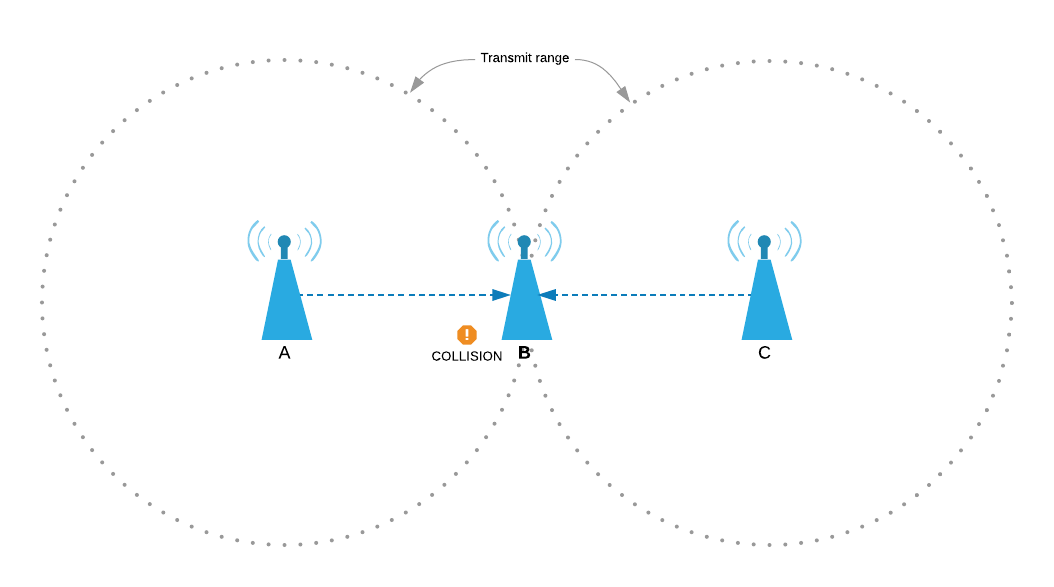
\includegraphics[width=13cm]{Images/HiddenTerminal.png} }}%

     \caption{The hidden terminal problem illustrated}
     \label{fig:hiddenterminal}
     \end{figure}


\section{Network infrastructure}
		This section provides a brief introduction to network infrastructures, to get an understanding of the differences between the mainly two types of infrastructures used today. 
		\subsection{Basic Service Set}
		A basic service set (BSS) in infrastruture mode consists of a single access point (AP) connected by wire to a distribution system (in residential deployment the distribution system is typically the ISP).
		Stations within the basic service area, which is the area physically serveable by the AP, can connect to the BSS using dynamic access point association, described
		in \cite{std80211}. A minimalist BSS infrastructure is illustrated in \ref{fig:basicserviceset}. It also worth mentioning that a BSS can also be configured to operate as an independent
		basic service set, where there is no infrastructure in place (no APs), and communication is direct between stations. This is more commonly known as ad-hoc mode.
		
		One basic service set per household is the typical infrastructure in residential networks, but it is not uncommon to have multiple basic service sets in larger homes,
		where APs are placed on different floors to have a better signal strength. Usually these APs have different service set identifiers (SSIDs), and each requires its own authentication.
		This is because the APs are not under the same extended service set. 

		 \begin{figure}
			 \center
			 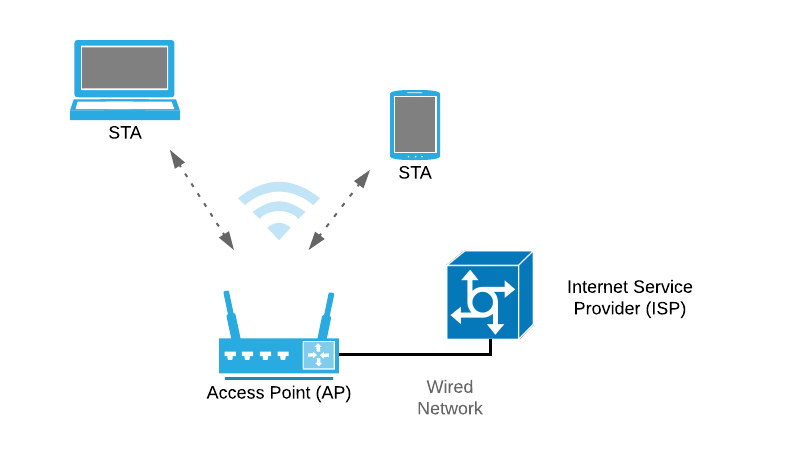
\includegraphics[scale=1]{Images/BSS.png}
			 \caption{Minimalist Basic Service Set in infrastructure mode}
			 \label{fig:basicserviceset}
		 \end{figure}

		\subsection{Extended Service Set}
		An extended service set (ESS) can consist of multiple basic service sets, and thereby APs. The extended service set is a logical entity which can extend station
		authentication and association to all APs under the same extended service set. In an ESS the SSID of all APs are also identical. This means a station (STA) can be in the basic service area of
		multiple APs at the same time, and is given the opportunity to select which AP to be serviced by. APs in an ESS can operate on different channels, and the medium access control
		mechanisms are performed as usual. Figure \ref{fig:extendedserviceset} illustrates the infrastructure of an extended service set.  

		 \begin{figure}
			 \center
			 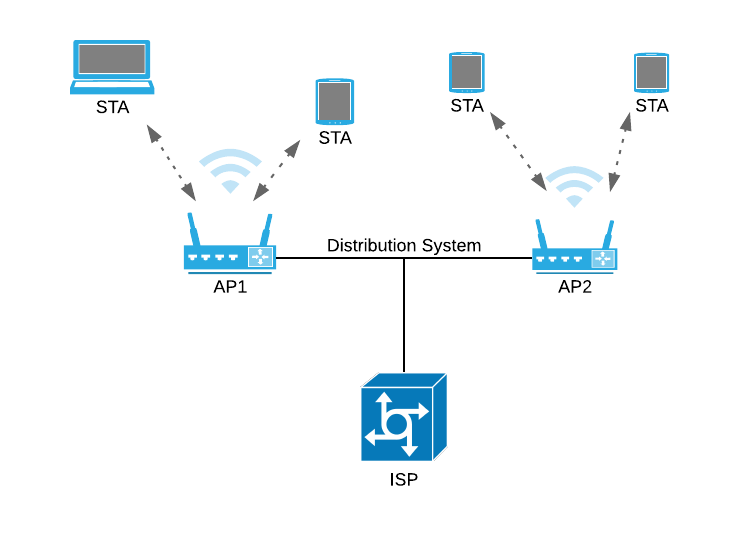
\includegraphics[scale=1]{Images/ESS.png}
			 \caption{Extended Service Set}
			 \label{fig:extendedserviceset}
		 \end{figure}


     \section{MAC Layer}
		 In this section parts of MAC layer of the 802.11 protocol is accounted for.  
     The 802.11 MAC layer implements the Carrier Sense Multiple Access / Collision Avoidance (CSMA/CA) protocol to control access to the medium.
     The CSMA/CA protocol is designed to operate in an entirely distributed fashion, where all stations connected to the same basic service set operates on
     the same frequency without coordinated timeslots. As suggested by the name of the protocol, there are two basic operations in the CSMA/CA protocol:
     \textbf{Carrier Sensing (CS)} and \textbf{Collision Avoidance (CA)}, both of which will be briefly described here.

     \subsection{Carrier Sense}
     In 802.11, carrier sensing (CS) is done in two ways
     \begin{itemize}
     \item \textbf{Physical carrier sensing} handled by the physical layer (PHY) as Clear Channel Assessment (CCA), which we will talk about in the PHY subsection.
     \item \textbf{Virtual carrier sensing} is a MAC layer mechanism in place to limit the number of times
     a node has to request CCA from the physical layer. When a valid 802.11 frame is decoded on a listening wireless network interface, it can read the duration of
     the transmission from the MAC header. The frame with a duration is called a Network Allocation Vector (NAV). When a NAV is received 
     the channel is marked as busy and the node will refrain from transmitting and also refrain from rechecking the channel for the duration of the NAV. 
     \end{itemize} 


     \subsection{Collision Avoidance}
CSMA/CA attempts to avoid collisions and is helpful in a network layout that includes hidden terminals. Request To Send/Clear To Send (RTS/CTS)
	is the function that allows CSMA/CA to some degree avoid the hidden terminal problem. By letting a node first ask the receiver if it is
	available for transmission (RTS), it prevents the node from sending the payload frame unless it receives Clear To Send (CTS) frame from the receiver first.
	The other mechanisms for collision avoidance are: 
	\begin{itemize}	
	\item \textbf{Interframe spacing} (IFS) is the amount of time the channel has to be idle before a sender can compete for channel access. 
	To give priority to certain frame types, different types of frames can have different types of interframe spacing. The type of IFS is usually 
	prefixed with the letter of the frame type. Organized by relative interval length, the differents IFS are:
	\begin{itemize} 
	\item Short IFS (SIFS), before ACK, RTS, CTS.  
	\item DCF Mode IFS (DIFS), before RTS frames (or DCF data frames if RTS/CTS is disabled)

	\end{itemize}
	\item \textbf{Exponential backoff} is what prevents two competing nodes from sending at the same time. When the channel is clear
	for DIFS time, a node has to wait another  random number of milliseconds before transmitting. This is called backoff.
	The amount of backoff is randomly chosen from a contention window (CW). The contention window has a low start size,
	called $CW_{\text{min}}$. A node draws a backoff time in the range $(0, 2^n*CW_{\text{min}})$, where $n$ is the number 
	of times the transmission has failed, beginning at $n=0$, and $CW_{\text{min}}<CW_{\text{max}}$.
	\end{itemize}

	\subsection{Distributed Coordination Function}
	The distributed coordination function is the main mode of operation in the 802.11 MAC layer, and is supposed to provide fair and reliable 
	transmission for all nodes on the same network. Figure \ref{fig:dcfmode} shows the 
	frame exchange that happens. Following the figure, the transmitter has to wait DIFS time, before drawing 
	a number from the contention window and backing off that amount.
	As no other transmissions has begun during this time, and the channel is
	still clear, the transmitter sends out an RTS frame. When received by the receiver
	it waits SIFS time before transmitting a CTS frame. The transmitter then sends his
	data frame, and waits for the ACK that indicates a successful transmission. The 
	RTS/CTS mechanisms introduces extra overhead and is sometimes turned off. The
	size of the payload and the number of stations on the network decides
	whether it is beneficial to have it on or off \cite{DCFanalysis}.



	\begin{figure}
	\center
	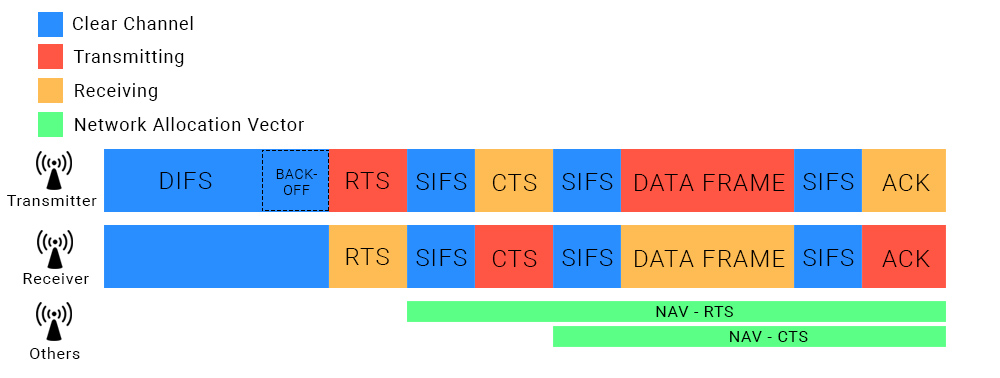
\includegraphics[scale=0.35]{Images/DCF.jpg}
	\caption{The timeline one frame transmission cycle in DCF mode}
	\label{fig:dcfmode}
	\end{figure}



	\section{PHY Layer}
	The physical layer in 802.11 is also divided in two sub-layers. The upper sub-layer is the Physical Layer Convergence Procedure (PLCP), responsible for clear channel assessment and acting
	as a common interface for MAC layer drivers. The lower sub-layer is the Physical Medium Dependent (PMD) which is responsible for modulation and directly interfaces with
	the radio. It is responsible for transmitting the complete frames, as well as receiving and decoding incoming frames. 

	\subsection{PLCP Protocol Data Unit}
	The physical layer convergence procedure creates PLCP Protocol Data Units (PPDUs), 
	that consists of 3 parts. The preamble, the header and the frame from the MAC layer
	called MAC Service Data Unit (MSDU), see figure \ref{fig:PPDU}. The frame structure
	has a long and short format, and changes a little bit for High Rate DSSS (HR-DSSS),
	but contains mostly the same fields.

	\begin{figure}
	\center
	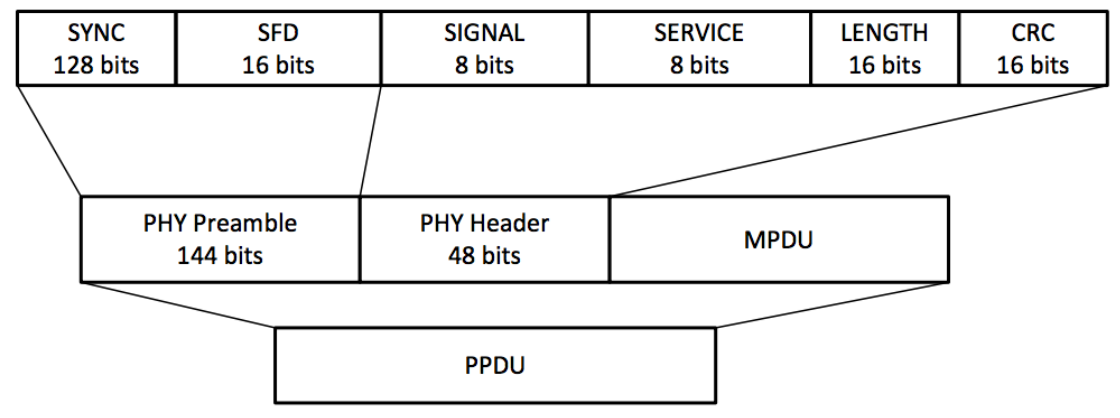
\includegraphics[scale=0.5]{Images/PPDU.png}
	\caption{DSSS PHY PPDU format from IEEE Std 802.11-2016  }
	\label{fig:PPDU}
	\end{figure}


	\begin{itemize}
	\item \textbf{Sync} bits are used to acquire the signal and synchronize timing. 
	\item \textbf{SFD} stands for Start Frame Delimeter and is there to indicate the start of a frame.  
	\item \textbf{Signal} the modulation type used to encode the MPDU and
	the data rate it is sent with. 
	\item \textbf{Service} Reserved for future use. 
	\item \textbf{Length} 16-bit fields that indicates the amount of time (in
			microseconds it will take to transmit the MPDU).
	\item \textbf{CRC} is the cyclic redundancy check that protects
	the fields signal, service and length. 
	\end{itemize}

	\subsection{Clear channel assessment}
	The PLCP layer provides clear channel assessment.
	The purpose of clear channel assessment is to give information to the MAC
	layer if the medium is available for transmission. There
	are primarily two ways the physical layer does CCA.
	\begin{itemize}
	\item CCA-ED (CCA-Energy Detect) detects signals that can not be decoded as a 802.11 frame, but is nonetheless a disturbing signal on the channel. If the CCA-ED value
	exceeds a threshold, for instance 20 dB, then the CCA shall be indicated as
	busy by issuing a \verb|PHY-CCA.indication(BUSY)| to the MAC layer.  
	\item CCA-CS (CCA Carrier/Sense) detects a valid 802.11 frame and can
	properly decode the header fields of a valid PPDU frame.
	The channel gets marked as busy for as long as the length
	field in the PPDU header specifies, even if the obvserved
	signal is weaker than the ED threshold. 
	\end{itemize}

	\section{Radio Frequency Interference}
	Radio Frequency Interference (RF-interference) is the result
	of two or more signals being transmitted on the same frequency at the same time.
	A receiver will have problems deciding which parts of the signals 
	belongs to which transmitter, and the signal may altered to the extent
	that bits are changed or misrepresented. As the 2.4 GHz band that 802.11
	utilizes is a part of the Industrial, Scientific and Medical (ISM) band, channel noise or interference
	can come from sources such as microwaves, bluetooth devices and radio controllers, in addition to other Wi-Fi devices. 

	\subsection{Impact in 802.11}
	If the PPDU header
	gets corrupted by an interfering signal and can not be decoded
	, the PLCP layer issues a \verb|PHY-RXEND.indication(CarrierLost)|
	to the MAC layer. According to CSMA/CA the station then has to
	wait EIFS (Extended Interframe Spacing) time before
	it can transmit a new frame. EIFS is defined as
	\verb|ACK transmission time + SIFS + DIFS.| This is because the station that received the corrupt frame have no idea if any neighbouring station
	received it correctly, and is about to transmit an ACK-frame in response. Additionally
	to waiting the minimum EIFS time, the station also has to wait for
	an idle channel indication from the PLCP layer again. 

	This is just the added delay if a collision happens. Of course, the more co-channel interference, the more transmitters are waiting for medium access, meaning
	the contention window will increase, and the frequency of which a transmitter is granted access to the medium will be reduced. Thus, interference is severely damaging for QoS on wireless networks.   % The correct formula for EIFS is $DIFS + SIFS + lowest transmission time" 

	\subsection{Countermeasures}
	Several countermeasures to limit the impact of RF-interference has been suggested.
	On the MAC layer there is frame aggregation with individual headers.
	Frame aggregation in 802.11n is a technique that wraps several payloads under the same
	header and send them together at the same time, once channel access is granted. This can improve the throughput
	if the channel is clear, but if the frame gets corrupted during transmission
	an increased amount of data is lost.
	Therefore it can be beneficial to aggregate a frame with individual headers.
	Even though this gives a slightly increased processing and transmission overhead
	compared to regular aggregation where there is no individual headers, 
	each frame can be selectively acknowledged.
	This means that only a few frames has to be retransmitted in case of corruption,
	and not the entire aggregation. 

	Additionally on the physical layer there are a couple of other suggested countermeasures:
	\begin{itemize}
	\item Changing the transmission power levels
	\item Lowering data rates
	\item Adjusting CCA threshold
	\item Forward error correction
	\item Changing packet sizes
	\end{itemize}


	\begin{wrapfigure}{R}{0.25\textwidth}
		\caption{\newline Channel distribution}
		\label{fig:channels}
		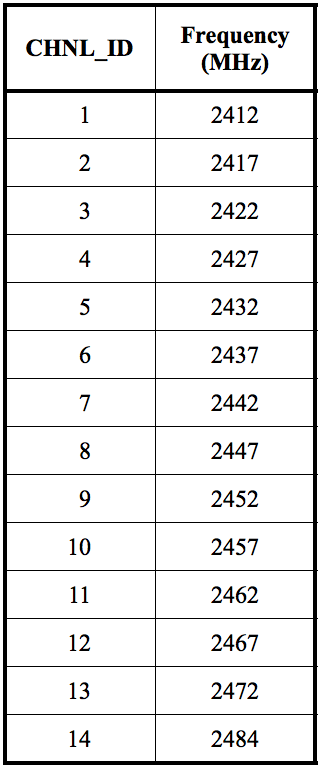
\includegraphics[width=1\linewidth]{Images/Channels80211.png}
	\end{wrapfigure}


	The mentioned countermeasures only have limited
	impact, while switching to a channel with less interference (if available) remains the most effective in most cases \cite{impactRF}. 
	\section{Channels} 
	802.11 b/g/n uses the range of frequencies from 2.400-2.500 GHz on the ISM band.
	The increasingly popular 802.11n/ac also uses a range of 5 GHz frequencies on the Unlicensed
	National Information Infrastructure (UNII) band, which offers more frequencies \cite{5ghz}.
	Other than that the properties and challenges for the different bands are ultimately the same.
	The distribution of the frequencies on the 2.4 GHz band to the different channels is illustrated by figure \ref{fig:channels}. The frequencies listed are the center frequencies of each channel. In practice this means that an AP that transmits on one channel will interfere with close channels in both directions. Two channels are entirely non-interfering if they send on two frequencies  $f_{1}$ and $f_{2}$ so that $|f_{1} - f_{2}| > 0.025$. This means that there are in total three completely non-overlapping channels, 1, 6 and 11. The process of deciding which channel to transmit on is called channel allocation. 




